\documentclass[a4paper, 11pt]{article}
\usepackage{comment} % enables the use of multi-line comments (\ifx \fi) 
\usepackage{fullpage} % changes the margin
\usepackage{color,listings,graphicx,float,booktabs,multirow, amsmath}
\usepackage[colorlinks=true, urlcolor=blue]{hyperref}

\definecolor{codegreen}{rgb}{0,0.6,0}
\definecolor{codegray}{rgb}{0.5,0.5,0.5}
\definecolor{codepurple}{rgb}{0.58,0,0.82}
\definecolor{backcolour}{rgb}{0.95,0.95,0.92}
 
\lstdefinestyle{mystyle}{
    backgroundcolor=\color{backcolour},   
    commentstyle=\color{codegreen},
    keywordstyle=\color{magenta},
    numberstyle=\tiny\color{codegray},
    stringstyle=\color{codepurple},
    basicstyle=\footnotesize,
    breakatwhitespace=false,         
    breaklines=true,                 
    captionpos=b,                    
    keepspaces=true,                 
    numbers=left,                    
    numbersep=5pt,                  
    showspaces=false,                
    showstringspaces=false,
    showtabs=false,                  
    tabsize=2
}
 
\lstset{style=mystyle}

\begin{document}
\graphicspath{{./figures/}}
\noindent
\large\textbf{Kyle Salitrik} \\
\normalsize CMPSC 450\\
\large{Homework 4 Report} \hfill 

%---------------------------------------------------------------
% Section 0
%---------------------------------------------------------------
\section*{Serial vs Parallel}
After adapting the CUDA code (ref: https://github.com/amosgwa/Exclusive-Scan-CUDA, https://developer.nvidia.com/gpugems/GPUGems3/gpugems3_ch39.html) to handle arrays larger than 1024, the program was set to run for M = 1000 to M = 10,000,000 in steps of 1000, where M is the size of the vector. Times were collected at the following sections in the code:
\begin{itemize}
	\item Before copying array to GPU
	\item Before running the GPU calculations
	\item After running the GPU calculations
	\item After copying the array from the GPU to the host
	\item Before running the serialized code
	\item After running the serialized code
\end{itemize}

This data is plotted in the figure below. Unsurprisingly, at low values of M, the serial computation is significantly faster due to the amount of time that it takes to copy the memory from the host to the GPU. However at around

\begin{figure}[H]
	\centering
	\centerline{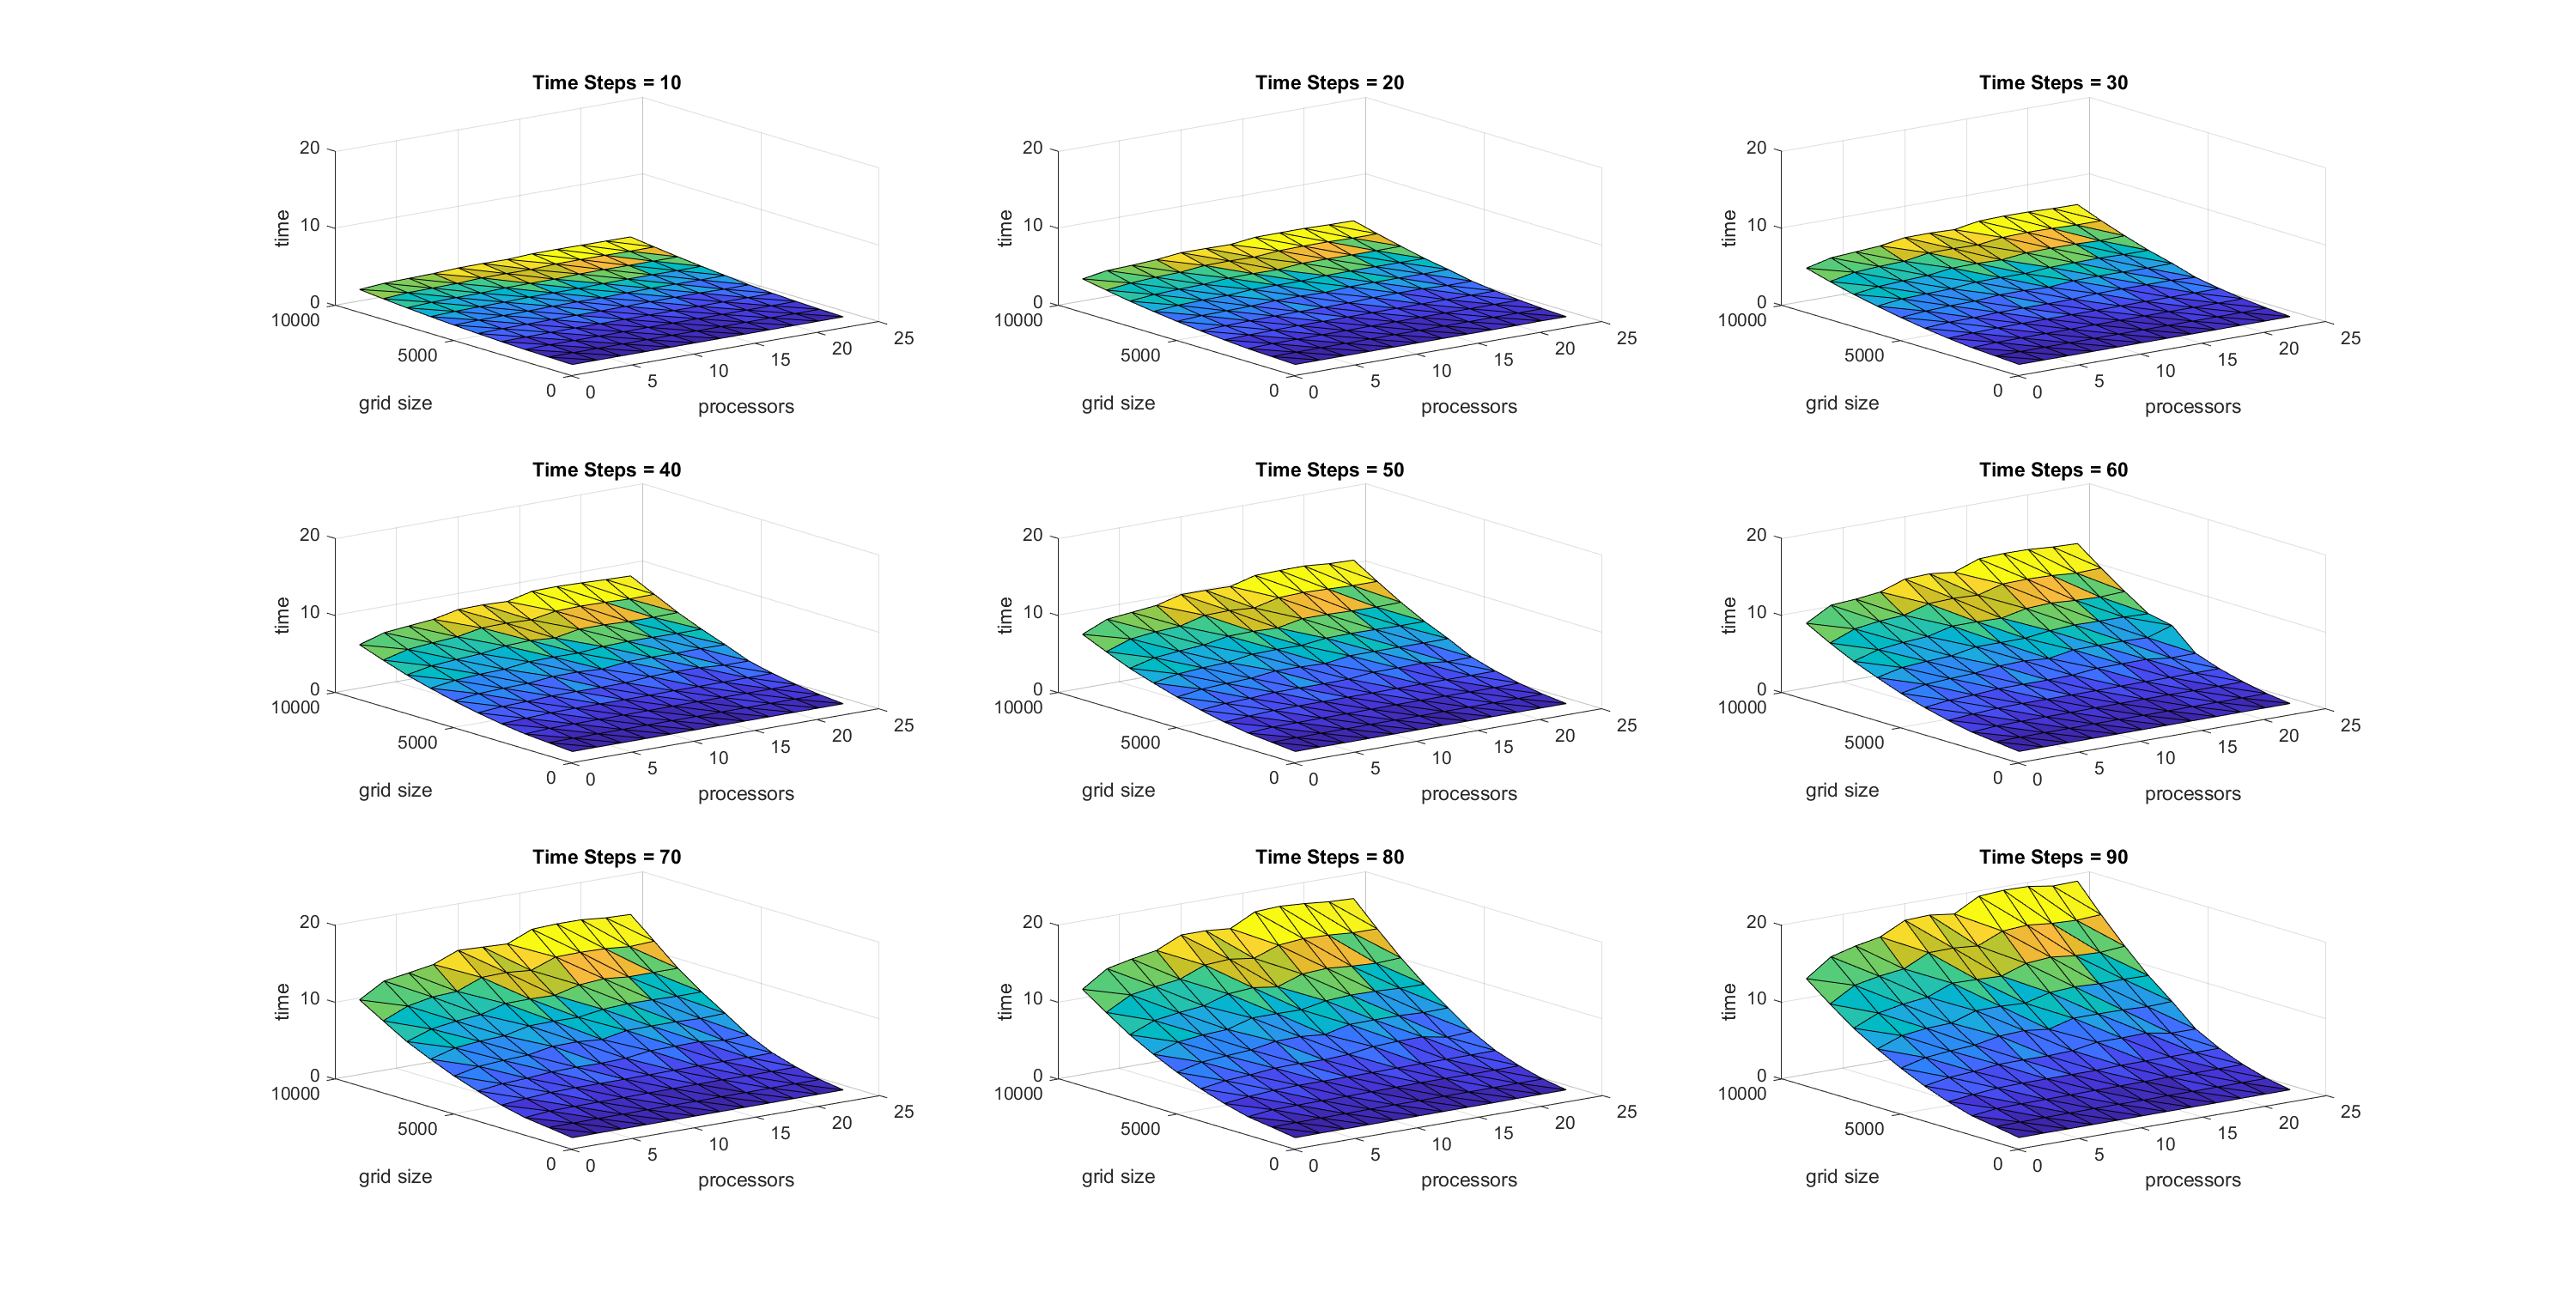
\includegraphics[width=7.5in]{comm_time_avg_scaled.png}}
	\caption{Average Communication Time for Given Time Steps (Adjusted)}
\end{figure}





%====================================================================
\newpage
\section*{Code Appendix}
\lstinputlisting[language=C]{../main.c}


\end{document}